\documentclass{article}
\usepackage{amsmath,amsthm,amssymb}
\usepackage {mathtext}
\usepackage{amsfonts} 
\usepackage[T1,T2A]{fontenc}
\usepackage[utf8]{inputenc}
\usepackage [english, russian] {babel}
\usepackage[babel=true]{microtype}
\usepackage{caption}
\usepackage{subcaption}
\captionsetup[table]{position=t,justification=raggedleft,slc=off}
\setlength{\abovecaptionskip}{0pt}
\usepackage {geometry}
\usepackage{graphicx}
\geometry{margin=1in}
\title{Лабораторная работа №1.3.2 \\ Определение модуля кручения стержня статическим методом}
\author{Павел Рудачихин \\ Б04-507}
\date{16.10.2025}
\begin {document}
\maketitle{}
\section* {Аннотация} 

\hspace{4mm} В работе определяется модуль кручения и проверяется закон Гука. Исследуются погрешности проводимых измерений.

\textbf{Цель работы:} измерить углы закручивания в зависимости от приложенного момента сил, рассчитать модули кручения и сдвига при статическом закручивании стержня, убедиться в справедливости закона Гука.

\textbf{В работе используются:} стойка для кручения стержня, стержень исследуемого материала, лазерный указатель, шкала, набор грузов, штангенциркуль, микрометр, рулетка, весы.

\textbf{Методы:} 1) определение  углового  коэффициента  наклона  зависимости двух величин; 2) измерение геометрических размеров с помощью штангенциркуля и микрометра; 3) измерение массы тел с помощью весов; 4) измерение расстояния с помощью рулетки; 5) измерение изменения положения точки лазерного указателя с помощью линейки-шкалы.

\section* {Теоретические сведения}
\subsection* {Модуль сдвига}

\hspace{4mm} \textit{Деформация} в точке по определению равна $\varepsilon = \dfrac{ds}{dx} $, т.е. деформация - это относительное смещение двух точек, делённое на первоначальное расстояние между ними. Напряжение - сила, отнесённая к единице площади: $\sigma = \dfrac{F}{S} $. Если $ds$ перпендикулярен $dx$, то имеет место деформация \textit{сдвига} (см. рис. 1).

\begin{figure}[h!]
	\centering
	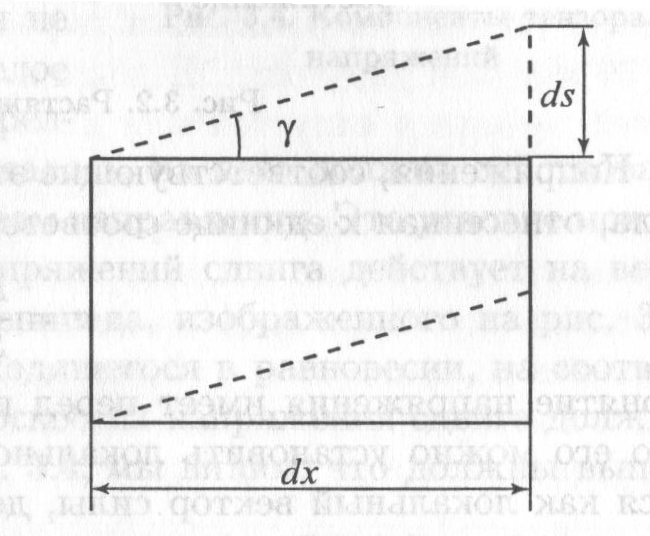
\includegraphics[width=0.3\linewidth]{1}
	\caption{Деформация сдвига}
	\label{fig:1}
\end{figure}


На основе эмпирических данных получено следующее соотношение для сдвига

\begin{equation} 
	\sigma = G\varepsilon,
\end{equation}

где $G$ -\textit{ модуль сдвига}.

Данное соотношение являются формой записи \textbf{закона Гука}, который справедлив для \textit{упругих} деформаций - устраняющихся при снятии внешней силы, вызвавшей деформации. Линейная зависимость сохраняется на интервале от нуля до некоторой предельной деформации. Далее имеет место \textit{необратимая}, или \textit{пластическая}, деформация.


\subsection* {Модуль кручения}

\hspace{4mm} При закручивании цилиндрических стержней круглого сечения распределение деформаций и напряжений одинаково по длине стержня только вдали от мест приложения закручивающих моментов. Для этих областей можно считать, что каждое поперечное сечение поворачивается как жёсткое. Такое напряжённое состояние называется \textit{чистым кручением}.

\begin{figure} [h!]
	\centering
	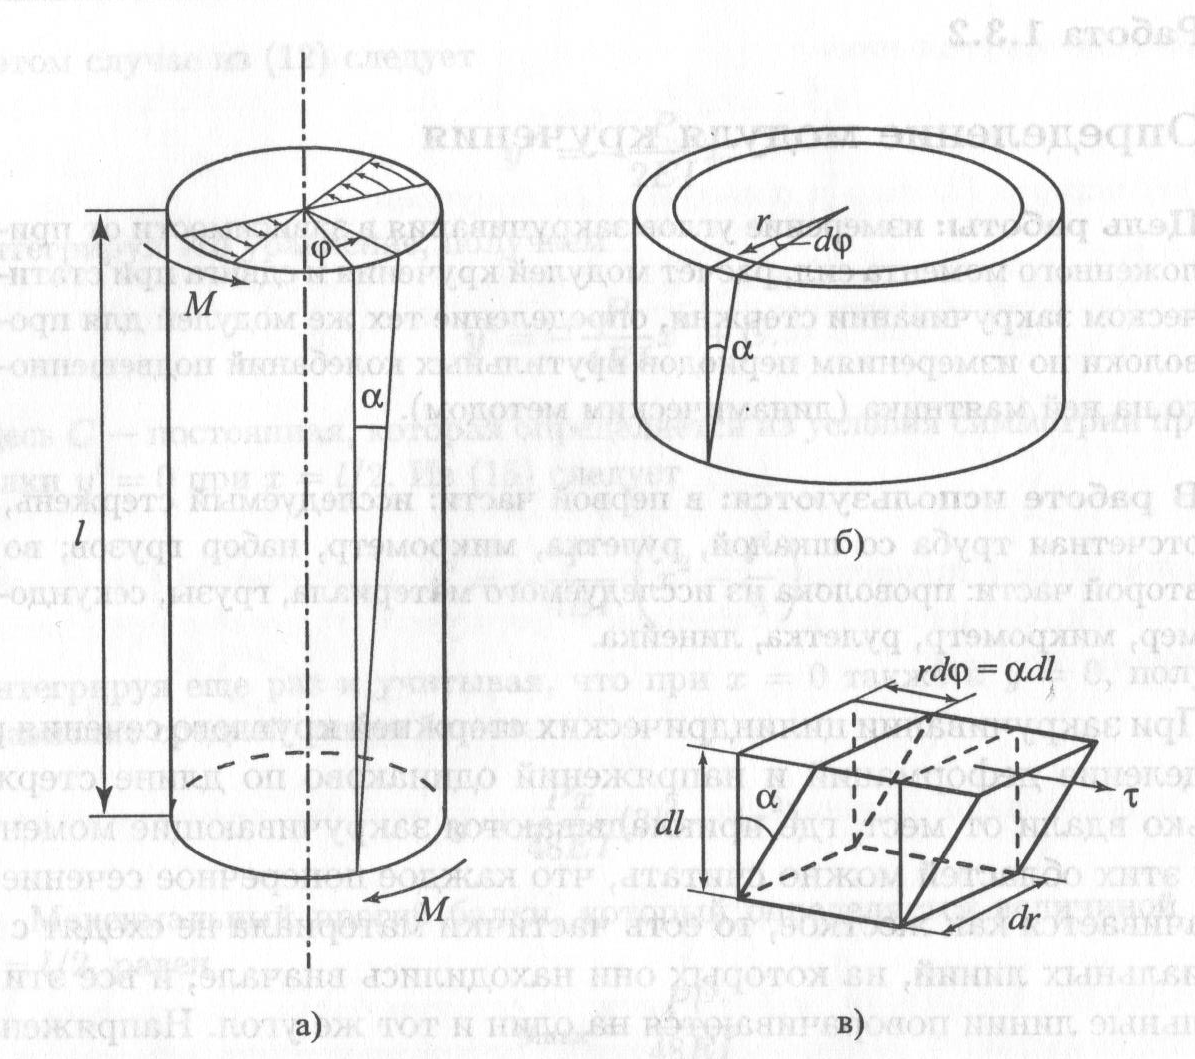
\includegraphics[width=0.4\linewidth]{2}
	\caption{Закручивание цилиндра}
	\label{fig:30}
\end{figure}


Любая прямая линия, параллельная оси симметрии стержня, при закручивании превращается в винтовую линию (см. рис. 2а). Сечения на расстоянии $l$ повёрнуты на угол $\varphi$. 

Рассмотрим кольцо произвольного радиуса $r$ малой толщины $dr$ и малой высоты $dl$ (см. рис. 2б). При закручивании верхнее сечение поворачивается относительно нижнего на угол $d\varphi$, цилиндрическая поверхность наклоняется на угол $\alpha$. При малых углах имеем:


\begin{equation}
	\alpha dl = rd\varphi
\end{equation}

В элементе кольца происходит деформация сдвига (см. рис. 2в). Касательное напряжение $\tau$ связано с углом сдвига через модуль сдвига $G$:

\begin{equation}
	\tau = G \alpha = G r \dfrac{d\varphi}{dl}
\end{equation}

Касательные напряжения связаны с моментом сил относительно оси цилиндра:

\begin{equation}
	dM = 2 \pi r\cdot dr \cdot \tau \cdot r
\end{equation}

Суммарный момент сил на всём поперечном сечении цилиндра:

\begin{equation}
	M = 2 \pi G \dfrac{d\varphi}{dl} \int_{0}^{R} r^{3} dr = \pi G \dfrac{d\varphi}{dl} \dfrac{R^{4}}{2} =  \dfrac{\pi G R^{4}}{2l} \varphi = f \varphi,
\end{equation}

где $f$ - модуль кручения.

\section* {Методика измерений}

\subsection* {Установка для статического закручивания стержня}

\hspace{4mm} Установка изображена на рисунке 3. С помощью системы из шкива Д, нитей Н и грузов Г к стержню приложен момент сил. 

\begin{figure}[h!]
	\centering
	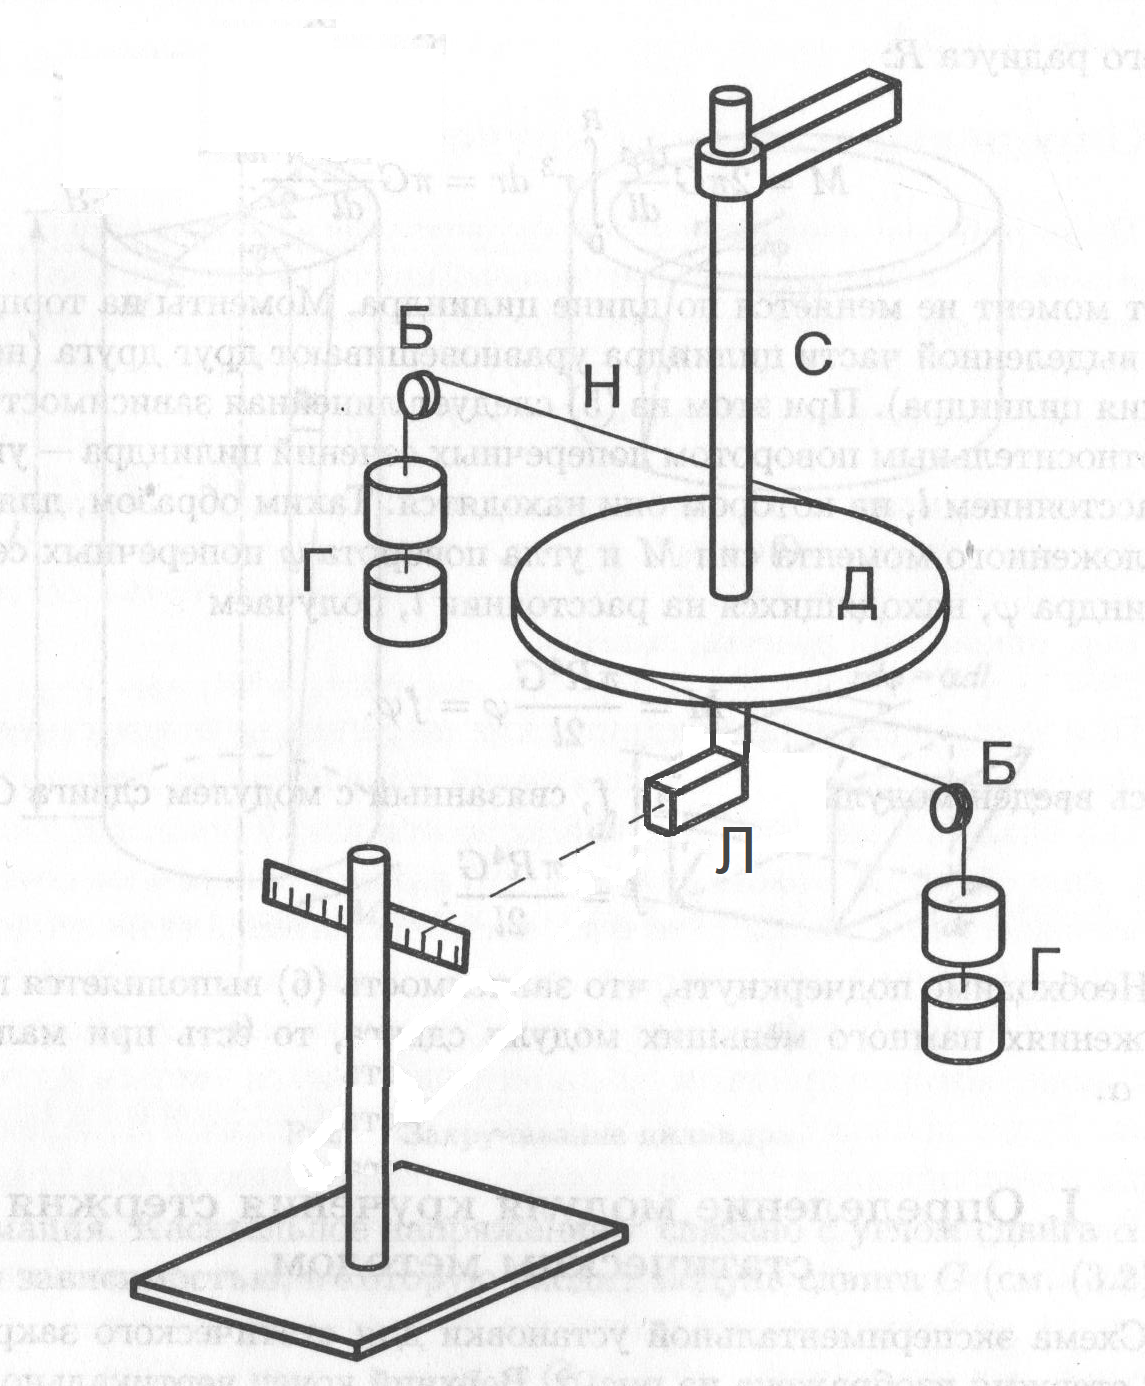
\includegraphics[width=0.4\linewidth]{3}
	\caption{\centering Установка для статического закручивания стержня: С - стержень, Н -нить, Б - блок, Д - шкив (диск), Г - груз, Л - лазерный указатель.}
	\label{fig:6}
\end{figure}

Если угол закручивания стержня мал, то его можно определить по метке лазерного указателя Л на шкале:

\begin{equation}
	\varphi \approx \tg \varphi = \frac{d}{L},
\end{equation}
где $d$ - положение метки, $L$ - расстояние от лазера до шкалы.

Считая нити нерастяжимыми и лёгкими, положим силу их натяжения равной силе тяжести, действующей на грузы. Тогда момент сил:

\begin{equation}
	M = M_1 + M_2 = m_1 g r + m_2 g r = (m_1 + m_2) g r,
\end{equation}

где $r$ - радиус шкива. 

\section*{Используемое оборудование}

\hspace{4mm} В данной работе для измерения массы использованы цифровые \textbf{весы}. Погрешность измерения массы определена как три в последнем разряде дисплея прибора: $\Delta_{\text{m}} = \pm 0,3$ г

Погрешность \textbf{линейки-шкалы} составляет $\Delta_{\text{Л}} = \pm 0,5$ мм 

Погрешность \textbf{штангенциркуля} определена маркировкой производителя: $\Delta_{\text{Ш}} = \pm 0,1$ мм

Погрешность \textbf{микрометра} определена маркировкой производителя: $\Delta_{\text{М}} = \pm 0,01$ мм

Погрешность \textbf{рулетки} определена ценой деления: $\Delta_{\text{Р}} = \pm 1$ мм


\section*{Результаты измерений}

\subsection*{Параметры установки}

\hspace{4mm} Параметры установки закручивания стержня приведены в таблице 1.  

\begin{table}[h!]
	\centering
	\captionbox{Параметры установки статического закручивания стержня}{
		\begin{tabular}{|c|c|}
			\hline
			Параметр  & Значение  \\
			\hline
			Длина стержня, $l$ & $(1330 \pm 2)$ мм \\
			\hline
			Диаметр шкива, $D$  & $(107,2 \pm 0,1)$ мм  \\
			\hline
			Расстояние от лазерного указателя до шкалы, $L$  & $(1540 \pm 1)$ мм \\
			\hline
			
	\end{tabular}}
\end{table}

Результаты измерений диаметра стержня микрометром представлены в таблице 2.

\begin{table}[h!]
	\centering
	\captionbox{Измерение диаметра стержня}{
		\begin{tabular}{|r|r|r|r|r|r|r|r|r|}
			\hline
			$2R$, мм & 5,95     & 5,95     & 5,94     & 5,94     & 5,96     & 5,97     & 5,96     & 5,96 \\
			\hline
	\end{tabular}}
\end{table}

Зависимость положения лазерного указателя на шкале от массы грузов представлена в таблице 3.

\begin{table}[h!]
	\centering
	\captionbox{Зависимость положения метки от массы груза}{
	\begin{tabular}{|r|r||r|r||r|r||r|}
		\hline
		$m$, г     & $d$, мм    & $m$, г     & $d$, мм    & $m$, г     & $d$, мм    & $\sigma_m$, г \\
		\hline
		100,4    & 51       & 100,4    & 53       & 49,5     & 23       & 0,3 \\
		\hline
		200,5    & 104      & 200,5    & 103      & 100,1    & 53       & 0,4 \\
		\hline
		249,8    & 133      & 249,8    & 136      & 149,5    & 76       & 0,5 \\
		\hline
		300,5    & 160      & 300,5    & 159      & 249,6    & 134      & 0,6 \\
		\hline
		350,0    & 183      & 350,0    & 184      & 350,0    & 187      & 0,7 \\
		\hline
		300,5    & 158      & 300,5    & 161      & 249,6    & 134      & 0,6 \\
		\hline
		249,8    & 129      & 249,8    & 136      & 149,5    & 78       & 0,5 \\
		\hline
		200,5    & 101      & 200,5    & 105      & 100,1    & 55       & 0,4 \\
		\hline
		100,4    & 51       & 100,4    & 56       & 49,5     & 26       & 0,3 \\
		\hline
	\end{tabular}}
\end{table}

\section*{Обработка результатов}
\hspace{4mm} В последнем столбце таблицы 3 представлены погрешности измерений масс грузов. Она возрастает при добавлении грузов, т.к. итоговая масса есть сумма измеренных масс. Погрешность суммы определена по формуле:

\begin{equation}
	\sigma_{m_1 + m_2} = \sqrt{\sigma_{m_1}^{2} + \sigma_{m_2}^{2}}
\end{equation}

Последовательность добавления грузов выбрана таким образом, чтобы в каждом измерении массы огрузки по обе стороны шкива были равны, поэтому момент силы по формуле 7:

\begin{equation}
	M = 2 m g r
\end{equation}

Его относительная погрешность:

\begin{equation}
	\varepsilon_M =  \sqrt{\varepsilon_m^2 + \varepsilon_r^2}
\end{equation}

Относительная погрешность измерения угла вычислена по формуле:

\begin{equation}
	\varepsilon_\varphi =  \sqrt{\varepsilon_d^2 + \varepsilon_L^2}
\end{equation}

Все вычисления произведены с использованием программы, написанной специально для этих целей на языке программирования Python. Построение графиков выполнено с помощью модуля Matplotlib. Исходный код программы содержится в электронном приложении к работе.

\begin{figure}
	\centering
	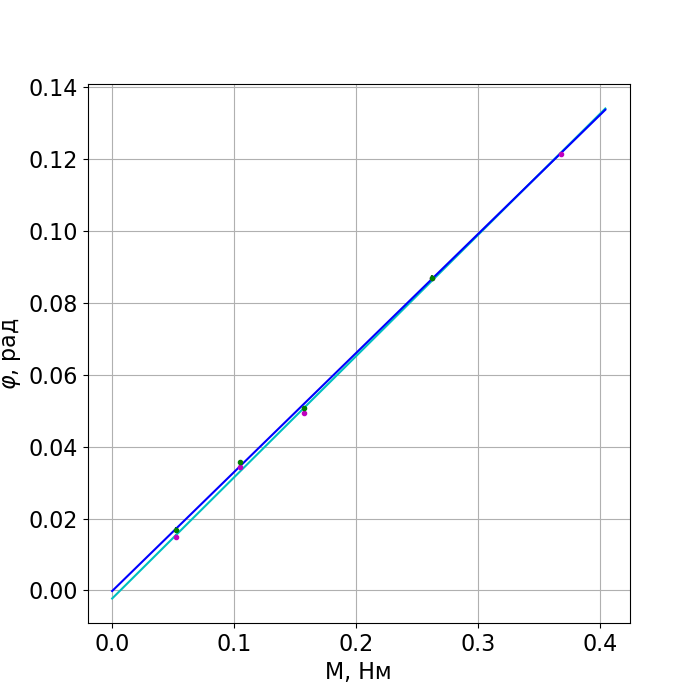
\includegraphics[width=0.6\linewidth]{3.3.0}
	\caption{\centering График зависимости $\varphi = \varphi(M)$ для возрастающей и убывающей последовательности грузов в третьем опыте (опыт с максимальным расхождением)}
\end{figure}




 Максимальная относительная погрешность измерения угла отклонения составила 3\%, измерения момента силы - 0,6\%. Для проведения прямой по экспериментальным точкам использован метод наименьших квадратов (см. рис. 5). 
 
 Проверено, что угловой коэффициент прямой при возрастании массы груза ($b = (0,337 \pm 0.004) \frac{\text{рад}}{\text{Н} \cdot \text{м}}$) мало отличается от такового при убывании ($b = (0,331 \pm 0.005) \frac{\text{рад}}{\text{Н} \cdot \text{м}}$) (см. рис. 4)

Результаты измерений модуля кручения в трёх опытах представлены ниже.

\begin{equation}
	\boxed{f_1 = (3,06 \pm 0,08) \frac{\text{Н} \cdot \text{м}}{\text{рад}}; \ \ f_2 = (3,02 \pm 0,07) \frac{\text{Н} \cdot \text{м}}{\text{рад}}; \ \ f_3 = (2,99 \pm 0,13) \frac{\text{Н} \cdot \text{м}}{\text{рад}}}
\end{equation}

\begin{figure}[h!]
	\centering
	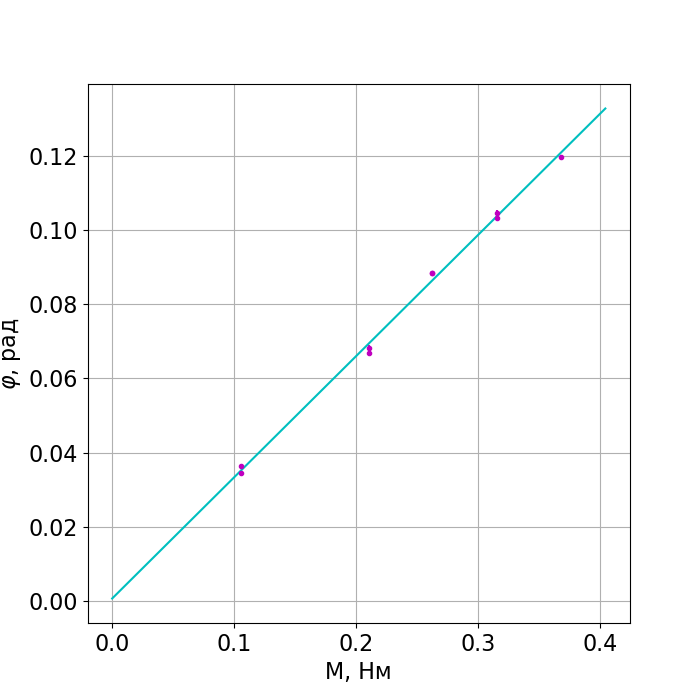
\includegraphics[width=0.3\linewidth]{3.1}
	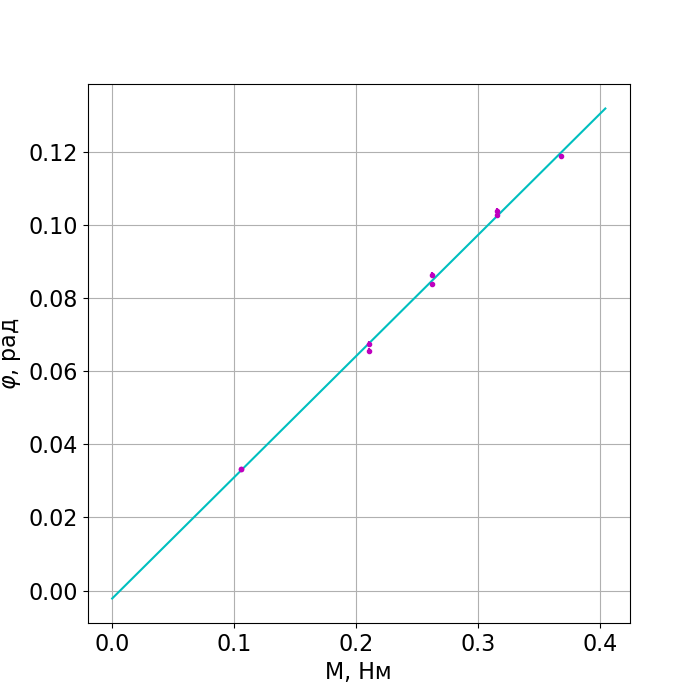
\includegraphics[width=0.3\linewidth]{3.2}
	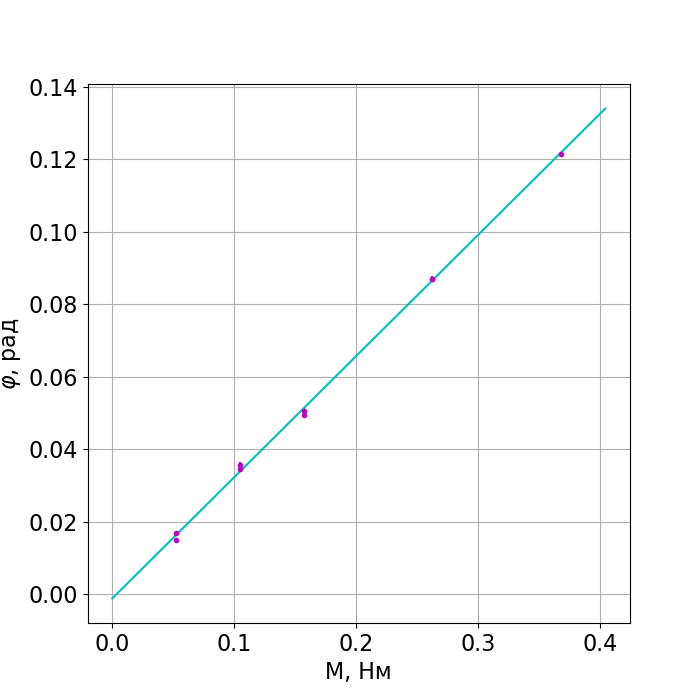
\includegraphics[width=0.3\linewidth]{3.3}
	\caption{\centering Графики зависимости $\varphi = \varphi(M)$ для трёх опытов}
\end{figure}

Для диаметра стержня ($D$) вычислены среднее значение, случайная и полная погрешности:

 \begin{equation}
 	\sigma_{сл} = \sqrt{\frac{1}{N} \sum_{i=1}^{N} (D_{i} - \langle D \rangle)^{2}} \ \ \ \
 	\sigma_{полн} = \sqrt{\sigma_{случ}^{2}+\sigma_{сист}^{2}}
 \end{equation}
 
 Радиус получается делением значения диаметра на два, погрешность радиуса определена умножением его значения на относительную погрешность измерения диаметра:
 
  \begin{equation}
 	R = (2,977 \pm 0,007) \ \text{мм}
 \end{equation}
 
 По формуле 5 выразим модуль сдвига:
 
 \begin{equation}
 	G  =  2 \dfrac{l f}{\pi R^{4}}
 \end{equation}
 
 Определим относительную погрешность модуля сдвига:
 
 \begin{equation}
 	\varepsilon_G = \sqrt{\varepsilon_l^2 + \varepsilon_f^2 + 16\varepsilon_R^2}
 \end{equation}
 
 Значения модуля сдвига для трёх опытов:
 
 \begin{equation}
 	\boxed{G_1 = (33,0 \pm 0,9) \text{ГПа}; \ \ G_2 = (32,6 \pm 0,8) \text{ГПа}; \ \ G_3 = (32,2\pm 1,4) \text{ГПа} }
 \end{equation}

\section*{Анализ результатов}

\hspace{4mm} Согласно справочным данным, модуль сдвига бронзы меняется в широких пределах и обычно составляет 33 - 37 ГПа \footnote[1]{А.Д. Гладун и др. Лабораторный практикум по общей физике - М.: МФТИ, 2012.}. Значения, полученные в работе, совпадают с ожидаемыми. 

Наибольший вклад в итоговую погрешность вносит измерение угла. Действительно, при смещении метки на 23 мм и инструментальной погрешности в 1 мм относительная погрешность измерения смещения превышает 4\%. Кроме того, толщина самой метки сравнима с ценой деления, что вносит дополнительную погрешность.

Отметим, что смещение метки, а значит и угол поворота стержня, не возвращается к исходному значению после снятия нагрузки, что говорит о возникновении необратимой деформации, которая не может быть учтена в измерениях и поэтому искажает их результаты. 

\section*{Заключение}
\hspace{4mm} Цели работы достигнуты: измерен модуль сдвига материала стержня; проверено, что зависимость деформации от напряжения носит линейный характер, т.е. закон Гука справедлив. Результат работы соотносится со справочными данными. Определены основные источники погрешностей.

\end {document}